\chapter{Plan of Action}
This project will take place over the whole span of this academic year with key milestones and deliverables planned to ensure steady progress and timely completion.

In the first semester, the focus will be on laying a solid foundation for the whole project. It will begin with extensive background reading on quantum computing and its applications. Concurrently, a literature survey will be conducted to dive deeper into the complicated process of optimising evolutionary quantum circuit design. This phase will also involve defining system requirements and conducting an analysis of the problem space.

After the first couple weeks, the project will enter its initial implementation stage where the basic GP framework alongside the quantum circuit simulation environments will be worked on. This will involve implementing basic genetic operations as well as establishing quantum circuit representation.

The second semester will primarily focus on optimisation of the GP algorithm. Rigorous testing and validation of the system will be conducted throughout this stage, as well as data collection for the final report. The final weeks will be devoted to documentation, result analysis and final report editing.

Throughout the duration of the project, regular meetings with my project supervisor will be scheduled in order to ensure the project will be completed on time and to address any issues or question that arise. The Gantt charts below provide a rough visual representation of the project timeline.

\begin{figure}[h!]
    \centering
    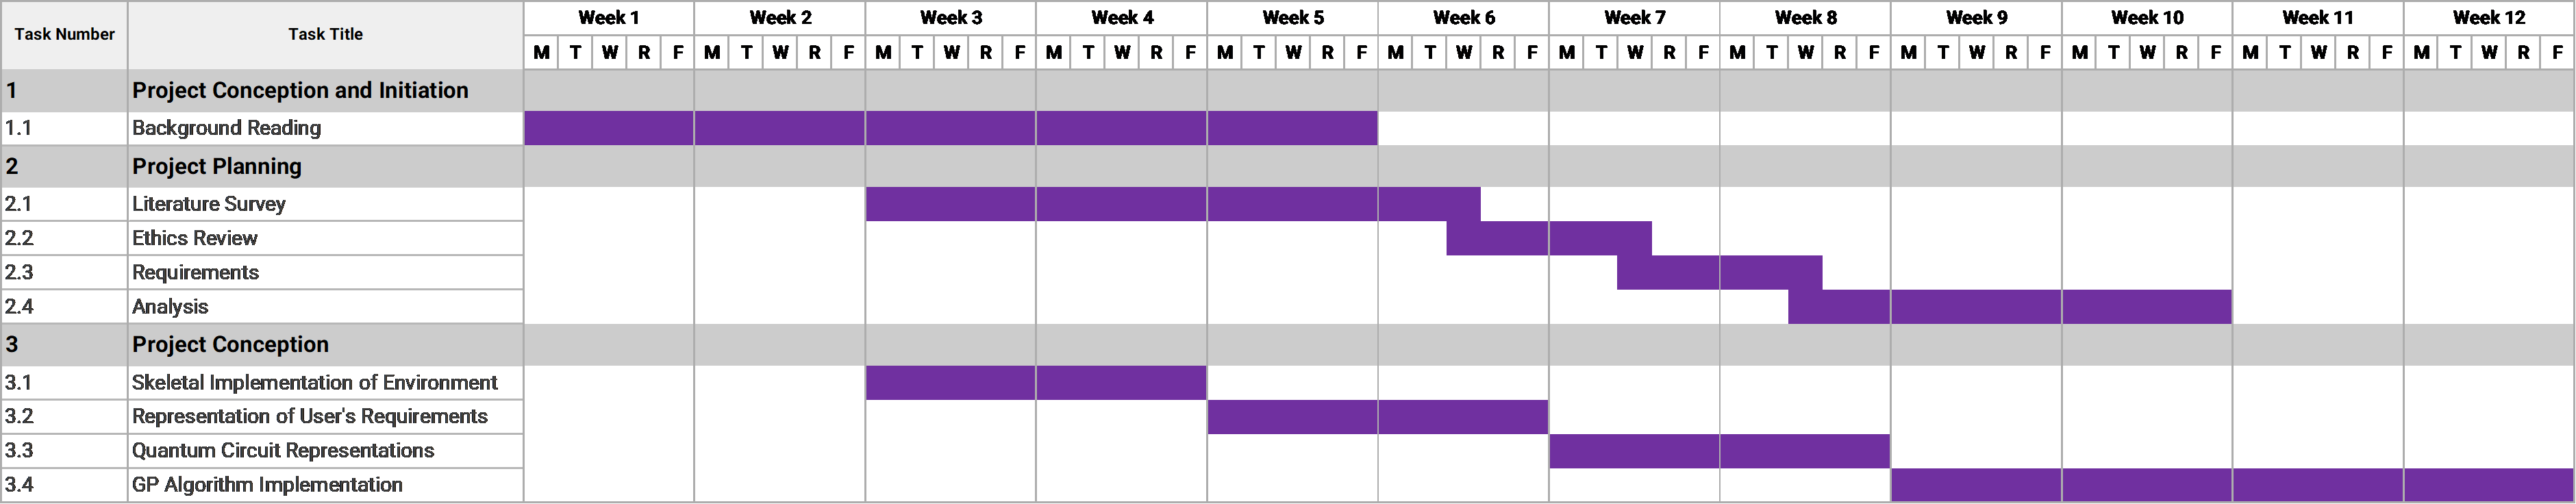
\includegraphics[width=\textwidth]{images/gantt_1.png}
    \caption{Gantt chart for semester one}
\end{figure}

\begin{figure}[t!]
    \centering
    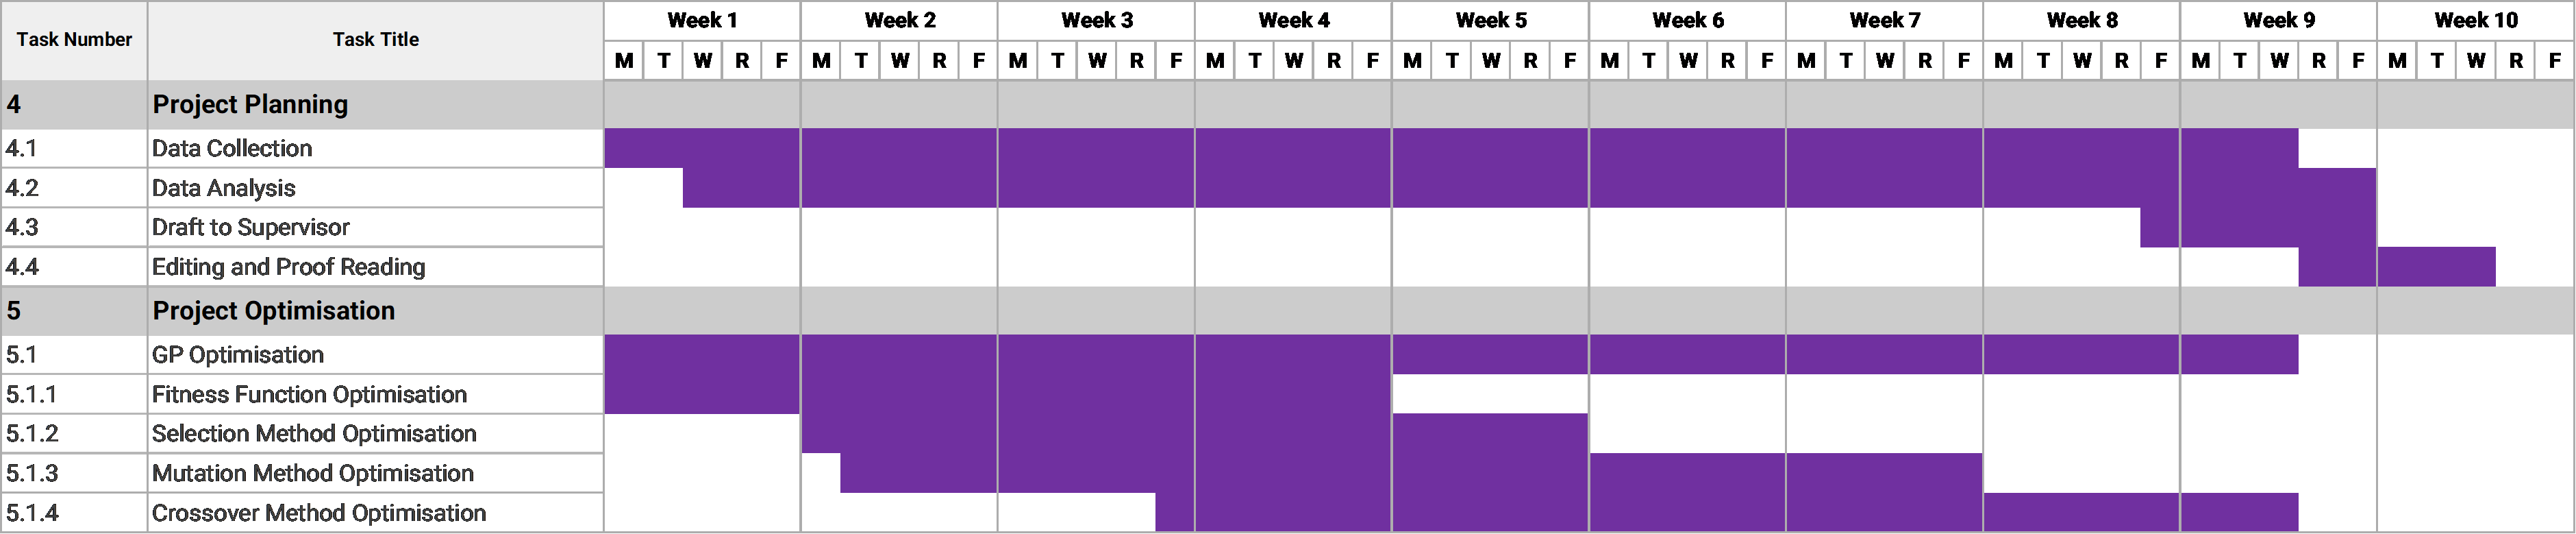
\includegraphics[width=\textwidth]{images/gantt_2.png}
    \caption{Gantt chart for semester two}
\end{figure}

% Chapter word count: 230
